% !TEX program = lualatex
\documentclass[11pt,a4paper]{article}

\usepackage[UTF8]{ctex} % 一句解决中文(含字体与断行等)

\usepackage{amsmath,amssymb,amsthm}
\usepackage{mathtools}
\usepackage{graphicx}
\usepackage{xcolor}
\usepackage{hyperref}
\usepackage{booktabs}
\usepackage{longtable}
\usepackage{array}
\usepackage{multirow}
\usepackage{siunitx}
\usepackage{enumitem}
\usepackage{csquotes}

% 代码相关:Pandoc 可能只认 verbatim/listings 一类;minted 依赖外部程序
\usepackage{listings}
\lstset{
  basicstyle=\ttfamily\small,
  breaklines=true,
  frame=single
}

% TikZ:Pandoc 通常不会“理解”TikZ,只会当 raw TeX
\usepackage{tikz}
\usetikzlibrary{arrows.meta,positioning}

% ---------- 自定义宏(Pandoc 的关键测试点) ----------
\newcommand{\R}{\mathbb{R}}
\newcommand{\E}{\mathbb{E}}
\newcommand{\norm}[1]{\left\lVert #1 \right\rVert}
\newcommand{\inner}[2]{\left\langle #1, #2 \right\rangle}
\newcommand{\vect}[1]{\mathbf{#1}}
\newcommand{\myemph}[1]{\textcolor{blue}{\textbf{#1}}}

% 带可选参数的宏(更“麻烦”)
\newcommand{\paren}[2][\big]{#1( #2 #1)}

% 自定义环境
\newtheorem{theorem}{Theorem}
\newtheorem{lemma}{Lemma}
\newenvironment{mybox}
  {\begin{center}\begin{tabular}{|p{0.85\linewidth}|}\hline}
  {\\\hline\end{tabular}\end{center}}

% ---------- 标题信息 ----------
\title{Pandoc LaTeX Stress Test}
\author{Someone}
\date{\today}

\begin{document}
\maketitle
\tableofcontents

\section{Text, Links, Footnotes, Quotes}

这是一段普通文本,包含强调 \emph{emph}、加粗 \textbf{bold}、等宽 \texttt{code},以及超链接:\href{https://pandoc.org}{Pandoc 官方站点}。

脚注示例\footnote{这是一个脚注。},以及引号:\enquote{quoted text}。

\begin{mybox}
	这是一个自定义环境 \texttt{mybox},里面也包含 \myemph{自定义宏渲染}。
\end{mybox}

\subsection{Percentages}

测试百分数:Test percent $100\%$ 和 100\%。

百分号在 $\LaTeX$ 中是注释符号,因此需要使用反斜杠进行转义以正确显示百分号符号;但并不需要美元符号包裹。

假设包裹,那么经过 CI 转换后仍然是:

\begin{verbatim}
$100\%$
\end{verbatim}

但在不同的环境下会有不同的表现:

\begin{itemize}
	\item VS Code 编辑器的 Markdown 预览中渲染正常。
	\item GitHub 上的 Markdown 渲染则不完整,显示为“100”后缺少百分号。
\end{itemize}

所以如果公式仅涉及百分号,建议直接写作“100\%”而非“$100\%$”。

\subsection{Lists}

无序列表:

\begin{itemize}
	\item 第一项
	\item 第二项,带数学 $a^2 + b^2 = c^2$
	\item 第三项,带自定义宏:$\norm{\vect{x}}$,$\inner{x}{y}$
\end{itemize}

有序列表(自定义格式):

\begin{enumerate}[label=(\alph*)]
	\item 选项 A
	\item 选项 B
\end{enumerate}

描述列表:

\begin{description}
	\item[Key] Value
	\item[Longer Key] A longer value text.
\end{description}

\section{Math}

行内数学:$\E[X]$,$\R^n$,以及可选参数宏:$\paren{t}$、$\paren[\Big]{t}$。

行间公式:

\[
	\int_0^1 x^2 \,dx = \frac 13.
\]

多行对齐:

\begin{align}
	f(x) & = x^2 + 1         \\
	     & = (x+1)(x-1) + 2.
\end{align}

带编号的定理环境:

\begin{theorem}[Pythagoras]
	For a right triangle, $a^2 + b^2 = c^2$.
\end{theorem}

\begin{lemma}
	If $x \in \R$, then $x^2 \ge 0$.
\end{lemma}

\section{Tables}

\subsection{Booktabs table}

\begin{table}[h]
	\centering
	\begin{tabular}{lS[table-format=3.2]r}
		\toprule
		Name  & {Value} & Note                   \\
		\midrule
		Alice & 12.34   & ok                     \\
		Bob   & 5.00    & \myemph{macro in cell} \\
		\bottomrule
	\end{tabular}
	\caption{A table with \texttt{booktabs} and \texttt{siunitx}.}
\end{table}

\subsection{Longtable}

\begin{longtable}{ll}
	\caption{A longtable example.} \\
	\toprule
	Key & Value                    \\
	\midrule
	\endfirsthead
	\toprule
	Key & Value                    \\
	\midrule
	\endhead
	A   & 1                        \\
	B   & 2                        \\
	C   & 3                        \\
	D   & 4                        \\
	\bottomrule
\end{longtable}


\subsection{Table with | in Math}

展示包含竖线的数学公式(绝对值):

注意:在纯 LaTeX 环境下,公式里直接用 | 是没问题的。但是如果使用了 | 作为绝对值符号,那么必然会在转换成 Markdown 表格的时候遇到问题,因为 Markdown 表格使用 | 作为列分隔符。

所以建议在数学公式中使用 \lvert 和 \rvert 来表示绝对值符号,例如 $\lvert x \rvert$。下面是一个示例表格:

\begin{table}[htbp]
    \centering
    \caption{Comparison of performance metrics across different models.}
    \label{tab:experiment_results}
    \begin{tabular}{l c c r}
        \toprule
        \textbf{Model Name} & \textbf{Accuracy (\%)} & \textbf{Loss Function} & \textbf{Time (ms)} \\
        \midrule
        Baseline Model      & 85.2\%                 & $\mathcal{L}_{CE}$     & 45.5 \\
        Method A            & 88.4\%                 & $|y - \hat{y}|$        & 102.0 \\
        \textbf{Ours (Pro)} & \textbf{92.1\%}        & $\|\Delta \theta\|_2$  & \textbf{38.2} \\
        \bottomrule
    \end{tabular}
\end{table}

\section{Figures}

图像(需要你放一个文件,如 \texttt{figures/demo.pdf}),CI 会尝试将其转换为 SVG。

\begin{figure}[h]
	\centering
	
\includegraphics[width=0.6\linewidth]{figures/demo.pdf}
	\caption{An included image.}
	\label{fig:demo}
\end{figure}

\section{Code Blocks}

\subsection{verbatim}

\begin{verbatim}
#!/usr/bin/env bash
echo "Hello, verbatim!"
\end{verbatim}

\subsection{listings}

\begin{lstlisting}[language=Python,caption={Python listing}]
def f(x):
    return x*x + 1
print(f(3))
\end{lstlisting}

\section{TikZ (raw TeX heavy)}

\begin{center}
	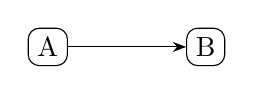
\begin{tikzpicture}[node distance=15mm]
		\node (a) [draw, rounded corners] {A};
		\node (b) [draw, rounded corners, right=of a] {B};
		\draw[-{Stealth}] (a) -- (b);
	\end{tikzpicture}
\end{center}

TODO: 将来会考虑生成 Tikz PDF 图,然后转换为 SVG 嵌入。

\section{Citations (BibLaTeX style placeholder)}

这里是引用占位:\cite{knuth1984texbook}。(如果你只用 Pandoc 读 LaTeX 转 Markdown,这一段通常会暴露“引用如何处理”的差异。)

% 你可以选择用 biblatex(LaTeX 编译):
% \usepackage[backend=biber,style=authoryear]{biblatex}
% \addbibresource{refs.bib}
% \printbibliography

\end{document}
